\documentclass[11pt,a4paper]{article}
\usepackage[margin=2.2cm]{geometry}
\usepackage[T1]{fontenc}
\usepackage{mathptmx}
\usepackage{booktabs}
\usepackage{graphicx}
\usepackage{amsmath}
\usepackage{caption}
\usepackage{float}
\usepackage[hidelinks]{hyperref}
\captionsetup{font=small,labelfont=bf}
\graphicspath{{../results/}}
\setlength{\parskip}{4pt}

\title{Risk-Aware Two-Way Auctions for AGV Dispatching\\at an Automated Container Terminal\\[4pt]
\large A discrete-event simulation study}
\author{Anwesh Ajitabh Dash\\\small B.Tech Mechanical Engineering, Vellore Institute of Technology\\
\small \url{https://github.com/Artianwe/agv-terminal-sim}}
\date{October 2026}

\begin{document}
\maketitle

\begin{abstract}
\noindent At an automated container terminal, a quay crane can only hand a container over when an automated
guided vehicle (AGV) is underneath it, so the dispatching of AGVs directly limits how fast a ship is
worked. I built a discrete-event simulation (Python, SimPy) of the waterside of a terminal with four quay
cranes, eight automated stacking cranes and 6--24 AGVs, and compared four dispatching policies: FIFO,
nearest vehicle, a centralised Hungarian-assignment controller and a decentralised Contract-Net auction.
The basic auction drives the least empty distance but loses up to 3.3 moves per crane-hour when vehicles
are scarce and about 1.5 when they are plentiful, because it commits jobs to busy vehicles on the basis of
over-confident arrival predictions. I propose a \emph{risk-aware two-way auction}: whichever side is
scarce makes the announcement, bids carry a safety margin learned online from past prediction errors, and
busy vehicles may only pre-commit when they can be on time and no idle vehicle can. Tuned on separate random
seeds and evaluated with common random numbers over 3,800 simulated vessel calls, it is never
significantly worse than the best benchmark at any fleet size, is significantly better than nearest vehicle at
14 AGVs (+0.23 moves/QC-h with 13\,\% less empty travel), and 12 AGVs (three per crane) are enough to
reach 90\,\% of crane capacity.
\end{abstract}

\section{Introduction}
Container terminals are multi-machine systems: quay cranes (QCs), horizontal transport and yard cranes
must work as one chain, and the slowest link sets the ship's handling time. In automated terminals the
horizontal link is usually a fleet of AGVs. Two design questions follow: \emph{how many AGVs} are needed
(fleet sizing), and \emph{how should they be dispatched} (which vehicle takes which container, and when)
\cite{steenken2004,leanh2006}. Classic dispatching rules are simple and robust \cite{egbelu1984};
centralised optimisation can do better but is a single point of failure and scales poorly
\cite{grunow2004,xin2014}. Multi-agent negotiation, such as the Contract Net Protocol \cite{smith1980},
is an attractive middle ground: each machine decides from local information.

This study asks: \emph{can AGVs negotiate jobs among themselves as well as a central controller assigns
them, across all fleet sizes?} Section~\ref{sec:model} describes the model, Section~\ref{sec:policies}
the policies, Section~\ref{sec:design} the experimental design, Section~\ref{sec:vv} verification and
validation, and Section~\ref{sec:results} the results.

\section{System and model}\label{sec:model}
\begin{figure}[H]
\centering
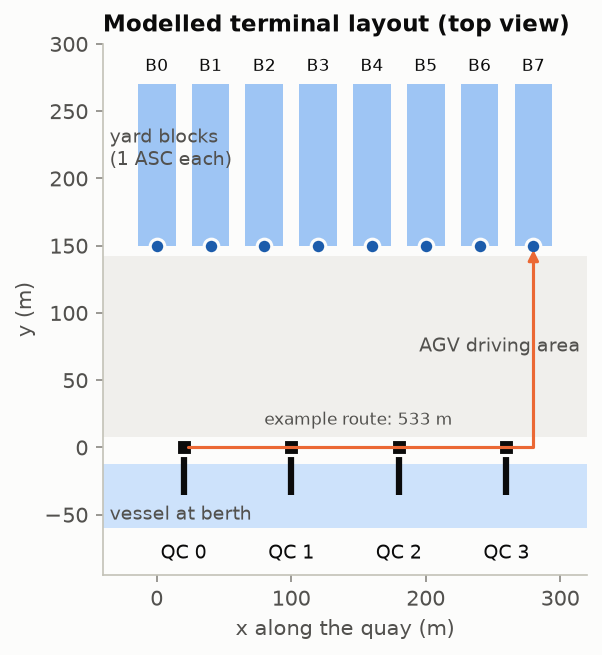
\includegraphics[width=0.52\textwidth]{fig_layout.png}
\caption{Modelled layout (top view): four QCs on the quay, eight yard blocks with one automated stacking
crane (ASC) each, and the AGV driving area in between.}
\label{fig:layout}
\end{figure}

One replication is one vessel call of 1,200 moves (4 QCs $\times$ 300). Even-numbered QCs discharge
first and then load; odd ones do the opposite, which creates chances for an AGV to drop one container at a
block and pick up the next one there. Each QC handles its job list strictly in order. A QC cycle is
triangular(70, 90, 130)\,s plus a 10\,s hand-over during which an AGV must be underneath; the QC
upper bound is therefore 33.8 moves per QC-hour. AGVs drive Manhattan routes $\times$ 1.3 at 5\,m/s plus
20\,s per leg, with lognormal noise (CV 0.1) and a Bureau of Public Roads congestion factor
$1+0.15\,(n_\text{moving}/20)^4$. Each ASC is a single server; the AGV waits during the transfer and,
for loads, while the ASC fetches the box. Each QC releases its next three jobs to dispatching. The model is
a terminating simulation, so no warm-up period is needed. Table~\ref{tab:params} lists the parameters and
where they come from.

\begin{table}[H]
\centering\small
\caption{Parameters and sources. ``Sensitivity'' marks values varied in Section~\ref{sec:sens}.}
\label{tab:params}
\begin{tabular}{p{3.9cm}p{3.4cm}p{7.9cm}}
\toprule
Parameter & Value & Source / argument \\
\midrule
QCs per vessel & 4 & as in \cite{gerrits2018} \\
QC cycle + hand-over & tri(70,90,130)\,s + 10\,s & mean 107\,s $\Rightarrow$ 33.8 moves/h; Jordan \cite{jordan2002}: 72\,s computed, $\approx$100\,s with yard delays; 22--30 moves/h gross in NW Europe \cite{saanen2003}; sensitivity \\
AGV speed & 5\,m/s cruise & max.\ 6\,m/s straight, 3\,m/s in bends, 2\,m/s$^2$ \cite{saputra2021} \\
Overhead per leg & 20\,s & acceleration/braking, two bends, positioning (10\,s in \cite{watson2005}) \\
Route factor & 1.3 & one-way lane loops vs.\ straight lines (assumption) \\
Quay-to-yard depth & 150\,m & assumption; sensitivity 100--250\,m \\
ASC transfer / store / retrieve & tri(20,30,45) / tri(40,60,90) / tri(40,60,90)\,s & $\approx$95\,s ASC time per move ($\approx$38 waterside moves/h); a single RMG with landside work does $\approx$30 moves/h \cite{watson2005}; sensitivity $\times$0.8--1.25 \\
Travel-time variability & CV 0.10 & assumption; sensitivity 0--0.3 \\
Congestion & BPR, $\alpha$=0.15, $\beta$=4, cap.\ 20 & standard BPR coefficients; sensitivity \\
Jobs released per QC & 3 & assumption; sensitivity 1--5 \\
\bottomrule
\end{tabular}
\end{table}

\section{Dispatching policies}\label{sec:policies}
All policies see the same released jobs and must assign each QC's jobs in sequence order, which rules out
deadlock (a unit test exercises deep commitment).
\begin{description}\itemsep2pt
\item[FIFO] oldest released job to the AGV that has been idle longest.
\item[Nearest vehicle] the idle-AGV/job pair with the shortest empty drive is matched first \cite{egbelu1984}.
\item[Central] whenever AGVs are idle, a Hungarian assignment \cite{kuhn1955} matches all idle AGVs to the released
jobs, minimising predicted hand-over time $+\,0.2\times$ empty drive time.
\item[Basic auction] the most urgent QC announces its next job; every AGV with fewer than two jobs bids its
own predicted hand-over time $+\,0.2\times$ empty drive time; the lowest bid wins \cite{smith1980}. Predictions
use mean times, the current ASC queue and a bias learned online (exponential moving average of errors).
\item[Risk-aware two-way auction (new)] three changes to the basic auction:
(i) \emph{two-way}: when released jobs outnumber idle AGVs, the idle AGV announces itself and takes the closest
job, as in the availability announcements of the Contract Net Protocol;
(ii) \emph{risk margin}: bids use $\max(\hat t_\text{arrive} + z\,\hat\sigma,\; t_\text{need})$, where
$\hat\sigma$ is the learned spread of past arrival errors, kept separately for idle and busy AGVs;
(iii) \emph{adaptive commitment}: a busy AGV may only win a job if its risk-adjusted arrival is on time
and no idle AGV is on time.
\end{description}

\section{Experimental design}\label{sec:design}
Each setting is replicated on 10 vessel calls (seeds 1--10). All random times are drawn before the run,
so every policy and fleet size sees identical containers and times (common random numbers). We report
means with Student-$t$ 95\,\% confidence intervals and compare policies by \emph{paired} per-seed
differences. The two settings of the new auction ($z$ and adaptive commitment) were chosen on separate
\emph{tuning} seeds 101--110 with a criterion fixed in advance: the smallest worst-case shortfall
(regret) in QC productivity relative to the best benchmark policy at each fleet size (Table~\ref{tab:tuning}).
The result, $z=2.5$ with adaptive commitment, was then frozen and evaluated on seeds 1--10.

\begin{table}[H]
\centering\small
\caption{Tuning on seeds 101--110 (best eight of 16 settings plus benchmarks), fleet sizes 6--24.}
\label{tab:tuning}
\begin{tabular}{lccc}
\toprule
Setting & Worst-case regret & Mean regret & Empty travel (m/move) \\
\midrule
Nearest vehicle & 0.08 & 0.02 & 137 \\
Risk-aware auction, $z=2.5$, adaptive commit on & 0.12 & 0.03 & 133 \\
Risk-aware auction, $z=3.0$, adaptive commit off & 0.13 & 0.06 & 125 \\
Risk-aware auction, $z=3.0$, adaptive commit on & 0.13 & 0.03 & 133 \\
Risk-aware auction, $z=2.5$, adaptive commit off & 0.17 & 0.06 & 122 \\
Risk-aware auction, $z=2.0$, adaptive commit on & 0.20 & 0.04 & 133 \\
Risk-aware auction, $z=2.0$, adaptive commit off & 0.21 & 0.10 & 120 \\
Risk-aware auction, $z=1.5$, adaptive commit on & 0.27 & 0.08 & 134 \\
\bottomrule
\end{tabular}

\end{table}

\section{Verification and validation}\label{sec:vv}
\textbf{Verification.} 23 automated tests check, among others: a hand-calculated deterministic case
(1 QC, 1 AGV: every hand-over time and the 751\,s makespan match exactly) for every policy; every job is
handled exactly once and in QC sequence; no deadlock with deep commitment; identical work plans across
policies (common random numbers); reproducibility; QC productivity never exceeds the crane's own cycle and
reaches it with a very large fleet; AGV time shares sum to one. The full experiment set was run on Linux and
on Windows~11 and the summary tables agree to $10^{-14}$.

\textbf{Validation.} Simulated QC productivity saturates at $\approx$32.8 moves/QC-h, close to the 34 moves/h
Gerrits et al.\ \cite{gerrits2018} simulated with 16 AGVs for 4 QCs and above the 22--30 gross moves/h
reported for NW European terminals \cite{saanen2003}, as expected for a model without landside work,
breakdowns or bay changes. Our knee of 3--4 AGVs per QC is below the 5.5 per QC suggested in
\cite{saanen2003}: our yard is close to the quay, traffic is represented only by a congestion function and
the QCs are single-hoist. The ranking of policies, not the absolute fleet size, is the robust output.

\section{Results}\label{sec:results}
\subsection{Fleet sizing}
\begin{figure}[H]
\centering
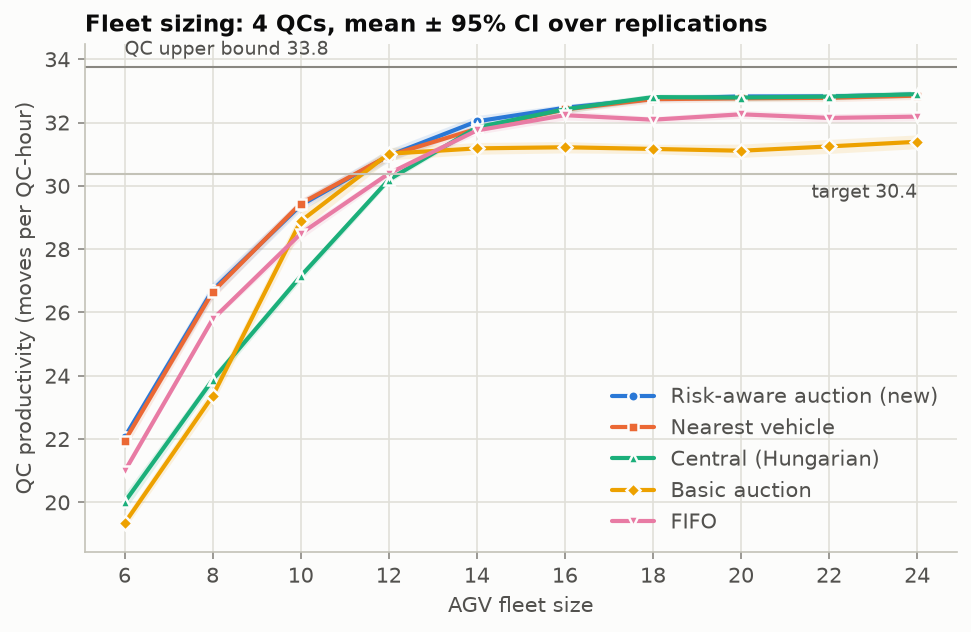
\includegraphics[width=0.78\textwidth]{fig_fleet_productivity.png}
\caption{QC productivity versus fleet size (mean $\pm$ 95\,\% CI, 10 vessel calls per point).}
\label{fig:fleet}
\end{figure}

\begin{table}[H]
\centering\scriptsize
\caption{QC productivity (moves per QC-hour, mean $\pm$ 95\,\% CI). Bold: best mean at that fleet size.}
\label{tab:fleet}
\begin{tabular}{rccccc}
\toprule
AGVs & Risk-aware auction & Nearest vehicle & Central (Hungarian) & Basic auction & FIFO \\
\midrule
6 & \textbf{22.05 $\pm$ 0.16} & 21.93 $\pm$ 0.26 & 20.01 $\pm$ 0.27 & 19.34 $\pm$ 0.18 & 20.98 $\pm$ 0.09 \\
8 & \textbf{26.71 $\pm$ 0.25} & 26.64 $\pm$ 0.22 & 23.87 $\pm$ 0.16 & 23.36 $\pm$ 0.25 & 25.78 $\pm$ 0.08 \\
10 & 29.39 $\pm$ 0.18 & \textbf{29.44 $\pm$ 0.15} & 27.14 $\pm$ 0.15 & 28.88 $\pm$ 0.29 & 28.49 $\pm$ 0.17 \\
12 & 30.95 $\pm$ 0.20 & 30.96 $\pm$ 0.15 & 30.19 $\pm$ 0.10 & \textbf{31.01 $\pm$ 0.19} & 30.39 $\pm$ 0.10 \\
14 & \textbf{32.04 $\pm$ 0.18} & 31.80 $\pm$ 0.11 & 31.85 $\pm$ 0.08 & 31.18 $\pm$ 0.19 & 31.75 $\pm$ 0.12 \\
16 & \textbf{32.47 $\pm$ 0.11} & 32.41 $\pm$ 0.11 & 32.42 $\pm$ 0.13 & 31.22 $\pm$ 0.18 & 32.23 $\pm$ 0.15 \\
18 & 32.75 $\pm$ 0.10 & 32.74 $\pm$ 0.12 & \textbf{32.80 $\pm$ 0.10} & 31.17 $\pm$ 0.15 & 32.09 $\pm$ 0.10 \\
20 & \textbf{32.82 $\pm$ 0.10} & 32.76 $\pm$ 0.10 & 32.79 $\pm$ 0.11 & 31.11 $\pm$ 0.21 & 32.26 $\pm$ 0.13 \\
22 & \textbf{32.83 $\pm$ 0.09} & 32.78 $\pm$ 0.12 & 32.82 $\pm$ 0.11 & 31.25 $\pm$ 0.22 & 32.15 $\pm$ 0.13 \\
24 & 32.89 $\pm$ 0.08 & 32.85 $\pm$ 0.12 & \textbf{32.90 $\pm$ 0.11} & 31.39 $\pm$ 0.22 & 32.19 $\pm$ 0.13 \\
\bottomrule
\end{tabular}

\end{table}

Three regimes appear (Fig.~\ref{fig:fleet}, Table~\ref{tab:fleet}). With 6--10 AGVs the vehicles are the
bottleneck and every metre of empty driving is lost capacity; rules that minimise it (nearest vehicle, the
two-way auction) are best, while urgency-driven rules (central, basic auction) lose 2--3 moves/QC-h. With
12--16 AGVs supply roughly matches demand and the policies differ most in how they use the little slack.
With 18 or more AGVs every policy except FIFO and the basic auction reaches $\approx$32.8 moves/QC-h.
For a 90\,\% target (30.4 moves/QC-h), 12 AGVs (three per QC) suffice with the new auction, nearest vehicle
or the basic auction, but the central controller needs 14; for 95\,\% all policies except the basic auction need 16.

\begin{table}[H]
\centering\scriptsize
\caption{Risk-aware auction minus each reference, paired over the same 10 seeds (mean $\pm$ 95\,\% CI).
$\Delta$ prod.\ in moves/QC-h; $\Delta$ empty in m per move (negative = less empty driving). Bold: significant.}
\label{tab:paired}
\begin{tabular}{rcccccc}
\toprule
& \multicolumn{2}{c}{vs nearest vehicle} & \multicolumn{2}{c}{vs central} & \multicolumn{2}{c}{vs basic auction} \\
AGVs & $\Delta$ prod. & $\Delta$ empty (m) & $\Delta$ prod. & $\Delta$ empty (m) & $\Delta$ prod. & $\Delta$ empty (m) \\
\midrule
6 & +0.12 $\pm$ 0.28 & +2 $\pm$ 3 & \textbf{+2.05 $\pm$ 0.32} & \textbf{-159 $\pm$ 6} & \textbf{+2.72 $\pm$ 0.28} & \textbf{-133 $\pm$ 3} \\
8 & +0.06 $\pm$ 0.23 & +1 $\pm$ 3 & \textbf{+2.83 $\pm$ 0.24} & \textbf{-116 $\pm$ 4} & \textbf{+3.35 $\pm$ 0.35} & \textbf{-90 $\pm$ 4} \\
10 & -0.05 $\pm$ 0.16 & +0 $\pm$ 3 & \textbf{+2.24 $\pm$ 0.20} & \textbf{-79 $\pm$ 3} & \textbf{+0.51 $\pm$ 0.35} & \textbf{-17 $\pm$ 4} \\
12 & +0.00 $\pm$ 0.16 & \textbf{+8 $\pm$ 4} & \textbf{+0.76 $\pm$ 0.14} & \textbf{-44 $\pm$ 2} & -0.06 $\pm$ 0.20 & \textbf{+33 $\pm$ 4} \\
14 & \textbf{+0.23 $\pm$ 0.14} & \textbf{-30 $\pm$ 11} & +0.19 $\pm$ 0.19 & \textbf{-43 $\pm$ 11} & \textbf{+0.85 $\pm$ 0.19} & \textbf{+85 $\pm$ 9} \\
16 & +0.05 $\pm$ 0.13 & \textbf{-10 $\pm$ 6} & +0.05 $\pm$ 0.09 & \textbf{-10 $\pm$ 5} & \textbf{+1.25 $\pm$ 0.17} & \textbf{+62 $\pm$ 4} \\
18 & +0.01 $\pm$ 0.10 & -2 $\pm$ 3 & -0.05 $\pm$ 0.07 & +0 $\pm$ 3 & \textbf{+1.58 $\pm$ 0.15} & \textbf{+12 $\pm$ 3} \\
20 & +0.06 $\pm$ 0.07 & +0 $\pm$ 3 & +0.03 $\pm$ 0.07 & +1 $\pm$ 4 & \textbf{+1.71 $\pm$ 0.23} & \textbf{+5 $\pm$ 4} \\
22 & +0.04 $\pm$ 0.10 & -1 $\pm$ 3 & +0.01 $\pm$ 0.07 & +0 $\pm$ 3 & \textbf{+1.58 $\pm$ 0.21} & \textbf{+4 $\pm$ 2} \\
24 & +0.04 $\pm$ 0.12 & +0 $\pm$ 2 & -0.01 $\pm$ 0.06 & +1 $\pm$ 2 & \textbf{+1.49 $\pm$ 0.22} & +3 $\pm$ 4 \\
\bottomrule
\end{tabular}

\end{table}

Table~\ref{tab:paired} is the main result. The risk-aware auction is never significantly worse than any
benchmark. Against nearest vehicle, the strongest benchmark, it is significantly better at 14 AGVs
(+0.23 moves/QC-h and 30\,m less empty driving per move) and equal elsewhere; against the central controller
it gains 0.8--2.8 moves/QC-h up to 12 AGVs; against the basic auction it gains 0.5--3.3 moves/QC-h at every
fleet size except 12, at the price of more empty driving in the 12--16 range.

\subsection{Why empty driving peaks at 14 AGVs}
\begin{figure}[H]
\centering
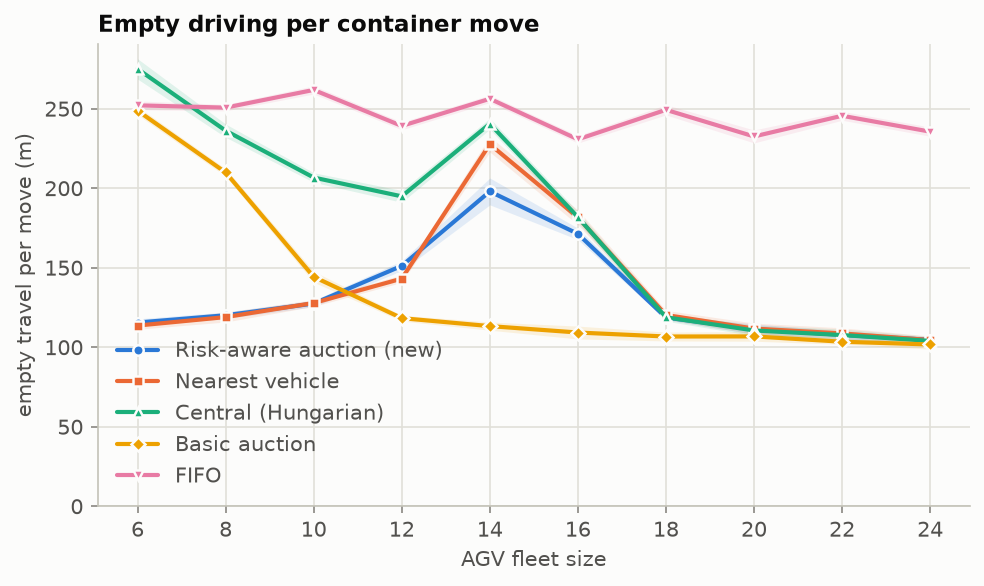
\includegraphics[width=0.49\textwidth]{fig_fleet_empty_travel.png}\hfill
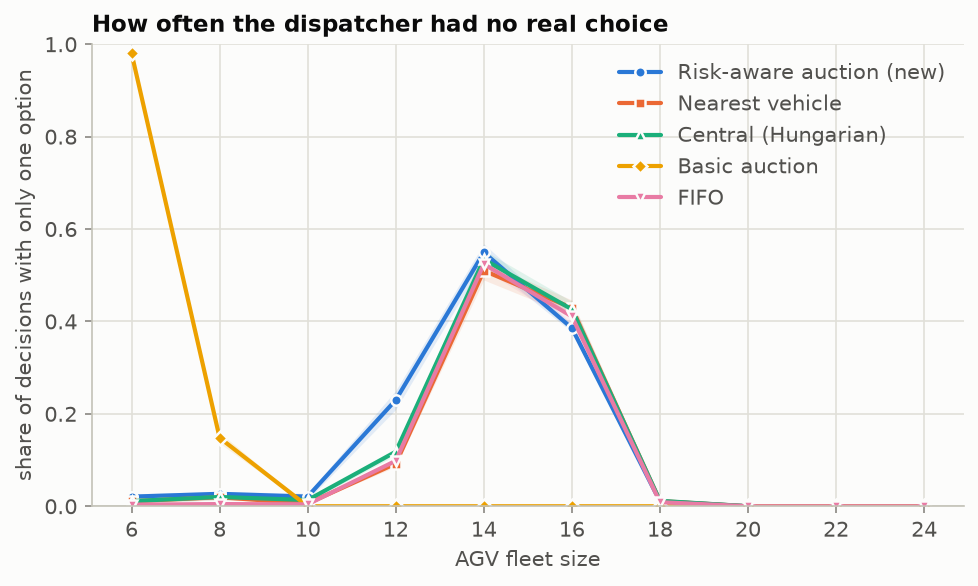
\includegraphics[width=0.49\textwidth]{fig_fleet_choices.png}
\caption{Left: empty travel per move. Right: share of dispatch decisions where only one option existed.}
\label{fig:choices}
\end{figure}
For idle-only policies, empty driving is not monotonic in fleet size: it peaks at 14 AGVs
(Fig.~\ref{fig:choices}). The right panel explains why: at that size supply $\approx$ demand, and about half of
all decisions have exactly one idle AGV and one job, so the dispatcher has no choice. With fewer AGVs, a freed
AGV can choose among up to four released jobs; with more, a job can choose among many idle AGVs.

\subsection{Ablation}
\begin{figure}[H]
\centering
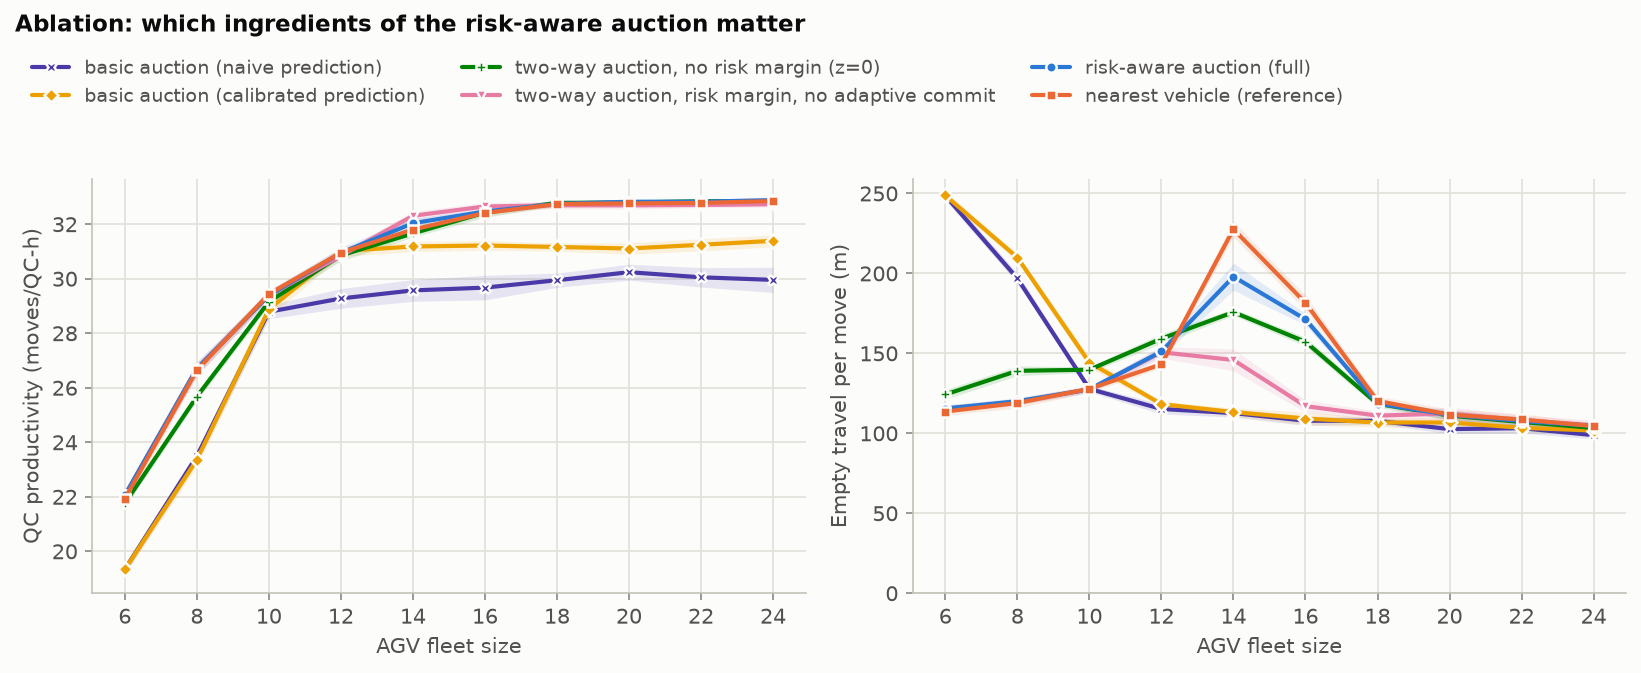
\includegraphics[width=\textwidth]{fig_ablation.png}
\caption{Ablation: switching on the ingredients of the risk-aware auction one at a time.}
\label{fig:ablation}
\end{figure}
Calibrated predictions alone lift the basic auction by 0.9--1.6 moves/QC-h at 14--24 AGVs. The two-way rule,
together with the on-time condition for busy AGVs, removes most of the remaining losses at both ends
(+2.4 moves/QC-h at 6 AGVs, +1.4 to +1.7 at 18--24). The learned risk margin adds a further 0.1--1.0 moves/QC-h
at 6--14 AGVs. Without adaptive commitment the auction drives less empty distance and is even slightly faster at
14--16 AGVs, but up to 0.16 moves/QC-h slower with 20 or more: a genuine efficiency--productivity trade-off,
which the worst-case tuning criterion resolved in favour of adaptive commitment (Fig.~\ref{fig:ablation}).

\subsection{Sensitivity}\label{sec:sens}
\begin{figure}[H]
\centering
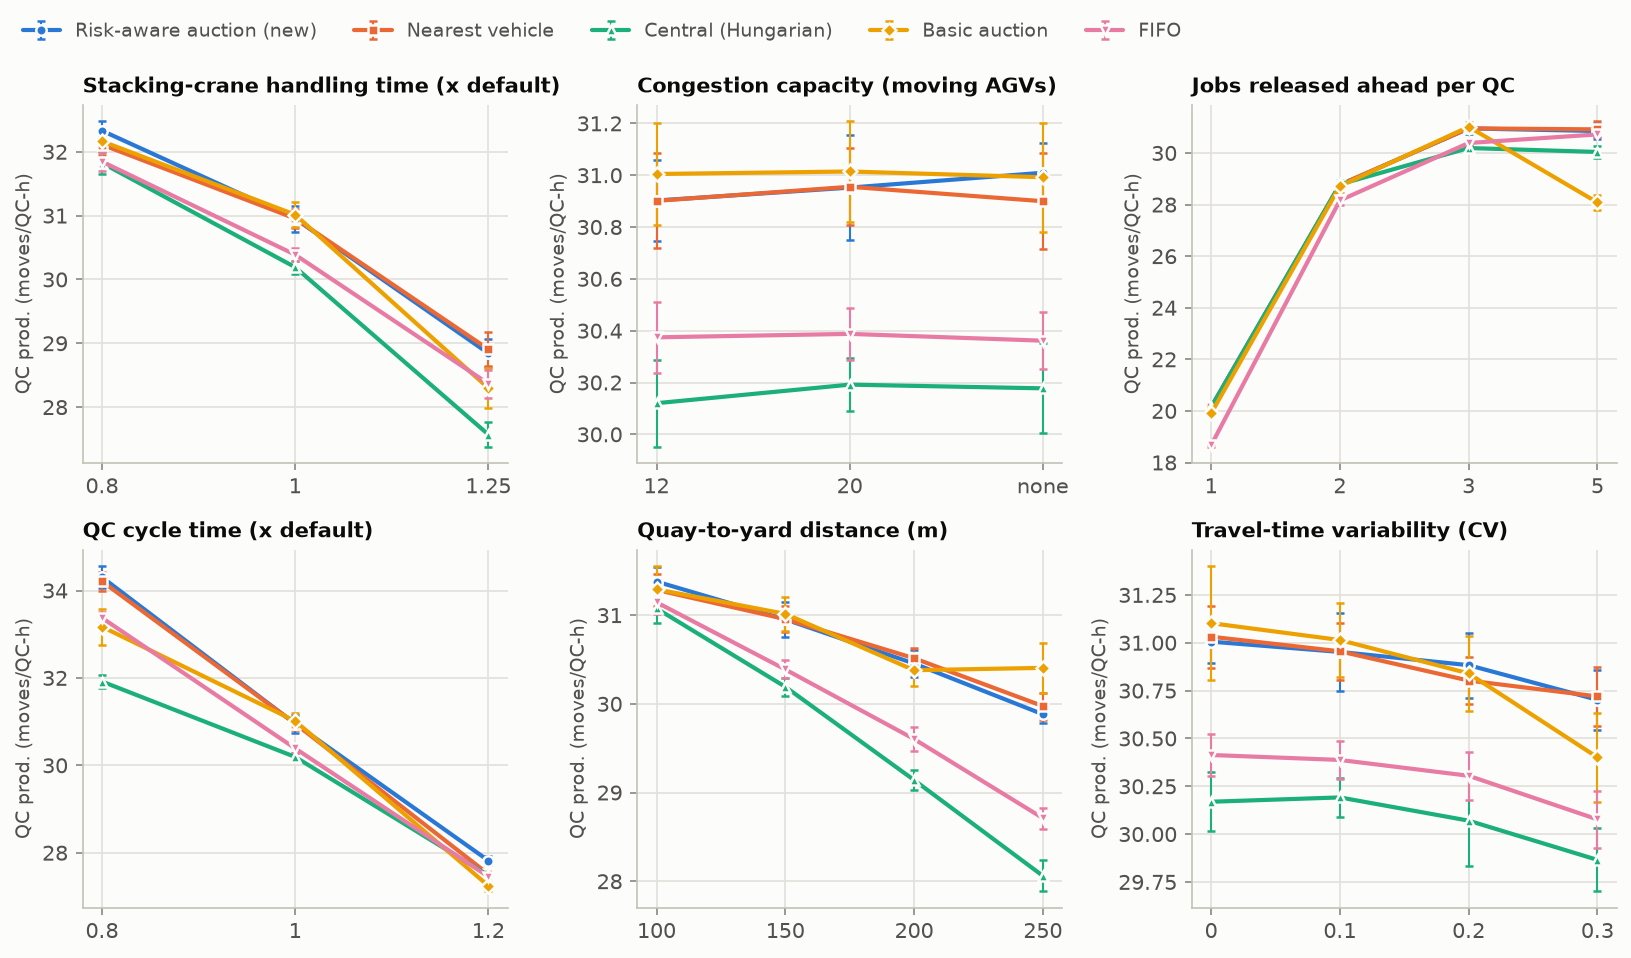
\includegraphics[width=\textwidth]{fig_sensitivity.png}
\caption{One-factor-at-a-time sensitivity at 12 AGVs.}
\label{fig:sens}
\end{figure}
The new auction stays within the confidence band of the best policy for every factor except the deepest yard
(250\,m), where the basic auction is about 0.5 moves/QC-h ahead (Fig.~\ref{fig:sens}). The basic auction is fragile when more
jobs are released ahead (lookahead 5: $-2.9$ moves/QC-h) and when travel times become more uncertain
(CV 0.3: $-0.7$); the risk-aware version loses only $-0.1$ and $-0.3$. The central controller degrades fastest with yard depth, because its
urgency-first assignment costs empty driving.

\begin{table}[H]
\centering\small
\caption{Policy comparison at 12 AGVs (mean $\pm$ 95\,\% CI).}
\label{tab:compare}
\begin{tabular}{lcccc}
\toprule
Policy & QC prod. (moves/QC-h) & Empty travel (m/move) & Crane wait (s/move) & Messages/job \\
\midrule
Risk-aware auction & 30.95 $\pm$ 0.20 & 151 $\pm$ 3 & 9.6 $\pm$ 0.7 & 31 \\
Nearest vehicle & 30.96 $\pm$ 0.15 & 143 $\pm$ 2 & 9.6 $\pm$ 0.4 & -- \\
Central (Hungarian) & 30.19 $\pm$ 0.10 & 195 $\pm$ 4 & 12.6 $\pm$ 0.4 & -- \\
Basic auction & 31.01 $\pm$ 0.19 & 118 $\pm$ 2 & 9.4 $\pm$ 0.8 & 10 \\
FIFO & 30.39 $\pm$ 0.10 & 239 $\pm$ 2 & 11.8 $\pm$ 0.3 & -- \\
\bottomrule
\end{tabular}

\end{table}

\section{Discussion and limitations}
A decentralised auction can match a centralised controller and a strong greedy rule \emph{if} the agents know
how uncertain their own predictions are and the protocol lets the scarce side speak first. Its cost is
communication: about 31 messages per container at 12 AGVs, roughly three times the basic auction
(Table~\ref{tab:compare}). Limitations: single-load AGVs; no explicit lanes, collision avoidance or traffic
deadlocks; random yard-block allocation; no battery charging; no buffer lanes or lift-AGVs at the crane; one
vessel and no landside traffic; ASCs do not pre-fetch; several parameters are assumptions (Table~\ref{tab:params}).
Natural next steps are an explicit lane network, energy-aware dispatching and testing the protocol under
communication delays and vehicle failures, the situations where decentralisation is meant to pay off.

\section{Conclusion}
Within this model, 12 AGVs (three per quay crane) give 90\,\% of crane capacity. A basic Contract-Net auction
is efficient but brittle. Adding a two-way announcement rule, learned risk margins and adaptive commitment makes
it as good as the best of four benchmarks at every fleet size from 6 to 24 and better in the critical
balanced regime, without a central controller.

\begin{thebibliography}{99}\small
\bibitem{steenken2004} D.~Steenken, S.~Vo{\ss}, R.~Stahlbock. Container terminal operation and operations research -- a classification and literature review. \emph{OR Spectrum} 26(1):3--49, 2004.
\bibitem{leanh2006} T.~Le-Anh, M.B.M.~De~Koster. A review of design and control of automated guided vehicle systems. \emph{European Journal of Operational Research} 171(1):1--23, 2006.
\bibitem{egbelu1984} P.J.~Egbelu, J.M.A.~Tanchoco. Characterization of automatic guided vehicle dispatching rules. \emph{International Journal of Production Research} 22(3):359--374, 1984.
\bibitem{grunow2004} M.~Grunow, H.-O.~G\"unther, M.~Lehmann. Dispatching multi-load AGVs in highly automated seaport container terminals. \emph{OR Spectrum} 26(2):211--235, 2004.
\bibitem{xin2014} J.~Xin, R.R.~Negenborn, G.~Lodewijks. Energy-aware control for automated container terminals using integrated flow shop scheduling and optimal control. \emph{Transportation Research Part C} 44:214--230, 2014.
\bibitem{smith1980} R.G.~Smith. The Contract Net Protocol: high-level communication and control in a distributed problem solver. \emph{IEEE Transactions on Computers} C-29(12):1104--1113, 1980.
\bibitem{kuhn1955} H.W.~Kuhn. The Hungarian method for the assignment problem. \emph{Naval Research Logistics Quarterly} 2:83--97, 1955.
\bibitem{gerrits2018} B.~Gerrits, M.~Mes, P.~Schuur. A simulation model for the planning and control of AGVs at automated container terminals. \emph{Proc.\ Winter Simulation Conference}, 2018.
\bibitem{saanen2003} Y.~Saanen, J.~van~Meel, A.~Verbraeck. The design and assessment of next generation automated container terminals. \emph{Proc.\ European Simulation Symposium}, 2003.
\bibitem{watson2005} J.~Watson. Comparison of three automated stacking alternatives by means of simulation. TBA white paper, 2005.
\bibitem{jordan2002} M.A.~Jordan. Quay crane productivity. Liftech Consultants, 2002.
\bibitem{saputra2021} R.P.~Saputra, E.~Rijanto. Automatic guided vehicles system and its coordination control for containers terminal logistics application. arXiv:2104.08331, 2021.
\end{thebibliography}
\end{document}
